% !TeX root = ../bachlor-arbeit.tex
It would be beneficial to train the inverse model $\mc D \rightarrow I$ in a tandem structure 
$I \rightarrow \mc D \rightarrow I'$ with a pre trained forward model.
This would circumvent the many-to-one problem and the network could even be trained on arbitrary functions as knowledge of the design parameters to a training spectrum are not necessary.
This combined model can easily be implemented as all the necessary modules are already there. A possible implementation is shown in figure \ref{fig:al:combined}.
However, this model can not be trained.
To understand why we need to go back to the concept of {\hyperref[eq:bg:back_prop]{Backpropagation}}.
During training the gradient of the cost function needs to propagate backwards through the network. To capture this mathematically we will identify the forward model in figure \ref{fig:al:combined} as the last layer $L$ in a combined network. Equation \eqref{eq:bg:back_prop} tells us we need to calculate
\begin{equation}
    \delta^L_j = \pdv{C}{a^L_j} \ \pdv{a^L_j}{z^L_j} \,.
\end{equation}

The first part $\partial C / \partial{a^L_j}$ is simple and only depends on the cost function. For example using \\
$C_\s{mse} = \sum_j \qty(a_j^L - y_j)^2$
the derivative is 
$\partial{C} / \partial{a^L_j} = 2 \qty(a_j^L - y_j)$.
However, the second part 
$\partial{a^L_j} / \partial{z^L_j}$,
the output of the last layer derived by the input to the last layer, is not easily accessible. Maybe not accessible at all if we consider the calls to the database and interpolation that happen during this step. The only way to train this combined tandem model is by replacing the forward model with something where we can access the gradient. This means training a second Neural Network to solve the forward problem.
\\

\indent
The Network has to generate the right spectrum to an input Design. Once again we will use convolutional layers, as the output neurons of this Network are spatially related. Another indication to try a convolutional architecture is that the NN's used to generate photorealistic Images, like Nvidea's StyleGan \cite{Karras2018}, also rely on convolutional layers and we can think of a transmission spectrum as a 1D image.

\begin{figure}[H]
    \floatbox[{
    \capbeside
    \thisfloatsetup{capbesideposition={right,top}}}]{figure}[\FBwidth]
    {\caption{
        A part of the algorithm described in section \ref{sec:algorithm} can be understood as a tandem model 
        $I \rightarrow \mc D \rightarrow I'$.
        This combined model receives a target spectrum and outputs its best reproduction of that spectrum $I'$. The notation is the same as in figure \ref{fig:al:algo}.
    }
    \label{fig:al:combined}}
    {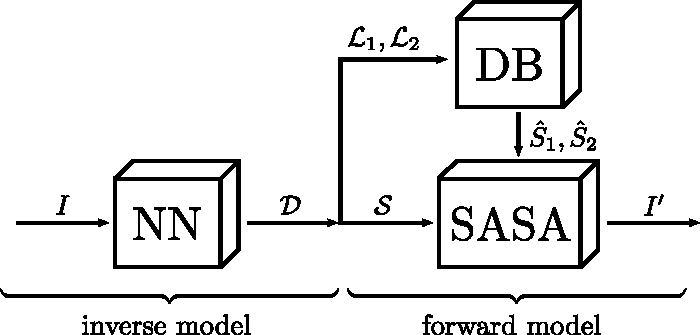
\includegraphics[width=0.6\textwidth]{al_combined}}
\end{figure}

\begin{figure}[H]
    \floatbox[{
    \capbeside
    \thisfloatsetup{capbesideposition={right,top}}}]{figure}[\FBwidth]
    {\caption{
        Example spectrum to viziulaize the effect of a running averge layer at the end of the forward model. 
    }
    \label{fig:in:avg_plot}}
    {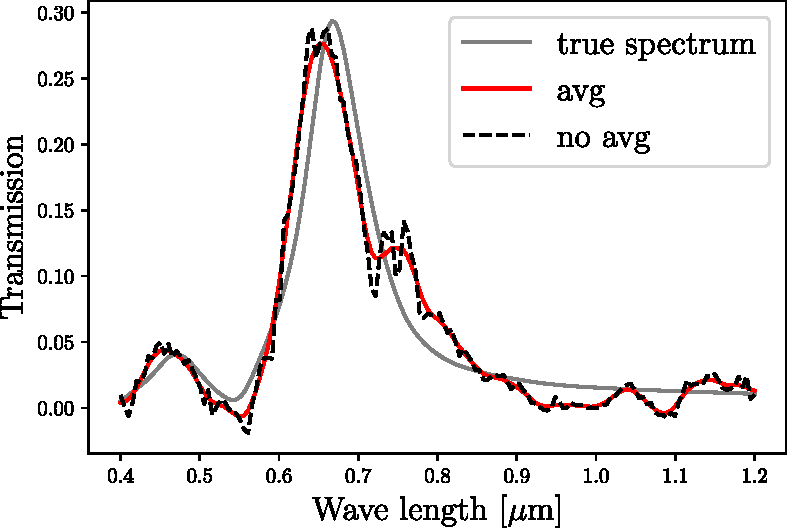
\includegraphics[width=0.57\textwidth]{in_avg_plot}}
\end{figure}